\section{Documento de diseño}
El juego que se obtendrá al final del desarrollo deberá cumplir con los requerimientos y características que se describirán en las siguientes secciones. Los requerimientos y características descritos deberán ser medibles y comprobables, ya que con base en ellos y con ayuda de diferentes pruebas se podrá comprobar el nivel de cumplimiento al que se llevaron.
%===========================================
	\subsection{Alcance}
	Los siguientes requerimientos son especificados para el juego Yolotl. El público objetivo del juego son jóvenes mexicanos mayores de trece años que cuenten con un teléfono móvil con sistema Android 5.1 instalado.   
%===========================================
	\subsection{Funcionalidad}
	La aplicación es un juego de plataformas de un solo jugador. El jugador controlará a un personaje durante la partida, mismo que podrá hacer evolucionar conforme avance en el juego.
	\\
	\par
La aplicación gestionara todas las acciones del jugador. De igual forma, la aplicación hará uso de un sistema de archivos para almacenar y controlar el progreso del jugador.
%===========================================
\subsection{Características de los usuarios.}
Al no manejar micro transacciones ni multijugador, la aplicación solo tendrá un perfil de usuario ver tabla \ref{tab:TipoUsuario}.
		%=======================		
		\begin{table} 
			\centering 
			\begin{tabular}{|l | c |} 
				\hline		
				\rowcolor{cyan}Usuario & Jugador\\ 
				\hline 
				Actividades & Iniciar partida, cargar partida, elegir nivel, jugar.\\ 
				\hline 
			\end{tabular}
			\caption{Usuario tipo juagdor y sus actividades que puede realizar dentro del juego.} 
			\label{tab:TipoUsuario}
		\end{table}
%===========================================
\subsection{Restricciones.}		
	\begin{itemize}
		\item Interfaz que se escale a las diferentes resoluciones de teléfonos móviles.
		\item El juego se desarrollará utilizando el motor gráfico Unity versión 6.6.2f1. Esta versión de Unity era la más reciente cuando se inició el proyecto. 
		\item El lenguaje bajo el que se desarrollará la aplicación será C $\sharp$.
		\item El juego será en 2D.
		\item El juego será para teléfonos móviles de gama media alta con sistema Android 5.1 instalado.
	\end{itemize}
%===========================================
\subsection{Requerimientos funcionales.}
	\begin{longtable}[c]{ | m{5cm} | m{10cm}|} 
		\hline
		\rowcolor{cyan}RF-001\label{RF:01} & Mostrar mensajes de confirmación. \\ 
		\hline
		Descripción	& El juego mostrará mensajes de confirmación para poder proceder con acciones que afecten de manera irreversible la partida del jugador. \\ 
		\hline
		Estado &  \\ 
		\hline
		Prioridad &  \\
		\hline
	%--------------------------------------------------
		\rowcolor{cyan}RF-002\label{RF:02} & Empezar partida. \\ 
		\hline
		Descripción	& El jugador podrá iniciar una partida nueva desde el menú principal del juego. \\ 
		\hline
		Estado &  \\ 
		\hline
		Prioridad &  \\
		\hline
		%--------------------------------------------------	
		\rowcolor{cyan}RF-003\label{RF:03} & Cargar partida.\\ 
		\hline
		Descripción	& El jugador podrá cargar una partida existente desde el menú principal del juego. \\ 
		\hline
		Estado &  \\ 
		\hline
		Prioridad &  \\
		\hline
		%--------------------------------------------------
		\rowcolor{cyan}RF-004\label{RF:04} & Seleccionar nivel a jugar. \\ 
		\hline
		Descripción	& El juego contará con un menú de selección de niveles en donde el jugador podrá seleccionar el nivel que desee jugar. \\ 
		\hline
		Estado &  \\ 
		\hline
		Prioridad &  \\
		\hline
		%--------------------------------------------------
		\rowcolor{cyan}RF-005\label{RF:05} & Desbloquear de Niveles. \\ 
		\hline
		Descripción	& El jugador desbloqueará niveles de manera secuencial, es decir, el nivel dos lo desbloqueara al finalizar el nivel uno. \\ 
		\hline
		Estado &  \\ 
		\hline
		Prioridad &  \\
		\hline
		%--------------------------------------------------	
		\rowcolor{cyan}RF-006\label{RF:06} & Controlar al personaje principal. \\ 
		\hline
		Descripción	& El jugador podrá controlar al personaje principal por medio de una interfaz gráfica de usuario. \\ 
		\hline
		Estado &  \\ 
		\hline
		Prioridad &  \\
		\hline
		%--------------------------------------------------	
		\rowcolor{cyan}RF-007\label{RF:07} & Mostrar cantidad de vida del jugador.\\ 
		\hline
		Descripción	& Cuando el jugador juegue un nivel, el juego le mostrará en tiempo real la cantidad de vida con la que dispone.  \\ 
		\hline
		Estado &  \\ 
		\hline
		Prioridad &  \\
		\hline
		%--------------------------------------------------	
		\rowcolor{cyan}RF-008\label{RF:08} & Mostrar cantidad de tonalli del jugador.\\ 
		\hline
		Descripción	& Cuando el jugador juegue un nivel, el juego le mostrará en tiempo real la cantidad de tonalli con la que dispone.  \\ 
		\hline
		Estado &  \\ 
		\hline
		Prioridad &  \\
		\hline
		%--------------------------------------------------	
		\rowcolor{cyan}RF-009\label{RF:09} & Mostrar el progreso de los objetivos del nivel.\\ 
		\hline
		Descripción	& En aquellos niveles con objetivos específicos como encontrar objetos, hablar con otros personajes, etc.; El juego le mostrará al jugador su progreso en tiempo real. \\ 
		\hline
		Estado &  \\ 
		\hline
		Prioridad &  \\
		\hline
		%--------------------------------------------------	
		\rowcolor{cyan}RF-010\label{RF:10} & Guardar progreso general del juego.\\ 
		\hline
		Descripción	& Al terminar un nivel el juego guardara de manera automática el progreso del jugador. \\ 
		\hline
		Estado &  \\ 
		\hline
		Prioridad &  \\
		\hline
		%--------------------------------------------------	
		\rowcolor{cyan}RF-011\label{RF:11} & Guardar progreso del juego dentro del nivel.\\ 
		\hline
		Descripción	& Dentro de los niveles existirán puntos de guardado llamados checkpoints. Estos puntos permitirán al jugador almacenar su progreso y volver a esa posición en caso de morir dentro de un nivel.\\ 
		\hline
		Estado &  \\ 
		\hline
		Prioridad &  \\
		\hline
	\end{longtable}
%===========================================
\subsection{Requerimientos no funcionales.}
	\begin{longtable}[c]{ | m{5cm} | m{10cm}|} 
		\hline
		\rowcolor{cyan}RNF-001\label{RNF:01} & Tiempos de carga. \\ 
		\hline
		Descripción	& Los tiempos de carga del juego no superaran los 10 segundos. \\ 
		\hline
		Estado &  \\ 
		\hline
		Prioridad &  \\
		\hline
	%--------------------------------------------------
		\rowcolor{cyan}RNF-002\label{RNF:02} & Inaccesibilidad de datos sensibles del juego. \\ 
		\hline
		Descripción	& El jugador no podrá modificar datos sensibles de la partida tal como la cantidad de vida, la cantidad de tonalli o los niveles disponibles \\ 
		\hline
		Estado &  \\ 
		\hline
		Prioridad &  \\
		\hline
		%--------------------------------------------------	
		\rowcolor{cyan}RNF-003\label{RNF:03} & Respeto a la privacidad.\\ 
		\hline
		Descripción	& El juego no recabara información del jugador. Al ser una aplicación para menores de edad, el juego basara su funcionamiento de manera offline.  \\ 
		\hline
		Estado &  \\ 
		\hline
		Prioridad &  \\
		\hline
		%--------------------------------------------------
		\rowcolor{cyan}RNF-004\label{RNF:04} & Tiempo de respuesta.\\ 
		\hline
		Descripción	& Cuando el jugador se encuentre jugando en un nivel, el juego responderá a las acciones del jugador en a lo más dos segundos.\\ 
		\hline
		Estado &  \\ 
		\hline
		Prioridad &  \\
		\hline
		%--------------------------------------------------
		\rowcolor{cyan}RNF-005\label{RNF:05} & Consistencia de frames. \\ 
		\hline
		Descripción	& El juego no presentara caídas de frames mientras se ejecute el juego en teléfonos móviles que cumplan con los requerimientos mínimos de funcionamiento. \\ 
		\hline
		Estado &  \\ 
		\hline
		Prioridad &  \\
		\hline
		%--------------------------------------------------	
		\rowcolor{cyan}RF-006\label{RNF:06} & Mantenibilidad. \\ 
		\hline
		Descripción	& La arquitectura del juego permitirá minimizar los tiempos de mantenimiento en caso de que se requiera actualizar el juego para componer errores que no se hayan detectado durante las pruebas.\\ 
		\hline
		Estado &  \\ 
		\hline
		Prioridad &  \\
		\hline
		
	\end{longtable}
%===========================================
\subsection{Casos de uso.}
En este apartado se describen los casos de uso del único actor que tiene el juego: el jugador. En la imagen se puede ver el diagrama de caso de uso del jugador.
%===========================================
\subsection{Reglas de negocio.}
A partir del documento de diseño se identificaron las siguientes reglas de negocio para el desarrollo del juego. 

\begin{longtable}[c]{ | m{5cm} | m{10cm}|} 
		\hline
		\rowcolor{cyan}Regla de Negocio & Descripción \\ 
		\hline
		%===================================
		RN-001\label{RN:01} & El juego solo permitirá una partida. \\ 
		\hline
		%===================================
		RN-002\label{RN:02} & La progresión dentro del juego será lineal. Es decir, el nivel n solo se desbloqueará si se ha completado el nivel n-1. Siendo el nivel 1 el que estará disponible por default.\\ 
		\hline
		%===================================
		RN-003\label{RN:03} & El archivo de datos de la partida usara un tipo de cifrado para evitar que el jugador lo pueda modificar.\\ 
		\hline
		%===================================
		RN-004\label{RN:04} & El personaje jugable durante los niveles 1 al 10 es el personaje de Malinalli. Sólo en el nivel 9, contará con otro personaje jugable además de Malinalli: Xólotl. \\ 
		\hline
		%===================================
		RN-005\label{RN:05} & Los niveles del juego ubicados en el Mictlán estarán divididos en dos etapas: una de plataformas y otra donde se deberá eliminar al guardián del nivel, salvo por el nivel 10. \\ 
		\hline
		%===================================
		RN-006\label{RN:06} & Existirán dos tipos de enemigos. Enemigos tipo normal y enemigos tipo Jefe. \\ 
		\hline
		%===================================
		RN-007\label{RN:07} & La información contenida en los checkpoints se mantendrá activa mientras el jugador se mantenga dentro del nivel. Una vez que el jugador sale del nivel esta información se elimina.\\ 
		\hline
		%===================================
		RN-008\label{RN:08} & La resolución que se manejará en los sprites será de 70 ppx.\\ 
		\hline
		%===================================
		RN-009\label{RN:09} & Los sprites solo contendrán colores en 8 bits.\\ 
		\hline
		%===================================
		RN-010\label{RN:10} & El jugador solo podrá dialogar con aquellos personajes que tengan un icono de dialogo. \\ 
		\hline
		%===================================
		RN-011\label{RN:11} & Los cuadros de diálogos solo contendrán  “” caracteres. En caso de que el dialogo exceda esa cantidad, el mensaje se dividirá en diferentes cuadros de diálogos hasta que se haya mostrado todo el mensaje. \\ 
		\hline
		%===================================
		RN-012\label{RN:12} & Cuando el jugador este dialogando con un personaje, la funcionalidad de los demás botones de la GUI se deshabilitarán.\\ 
		\hline
		%===================================
		RN-013\label{RN:13} & El jugador cuenta con una cantidad de tonalli determinada en cada disparo se gasta una cantidad por disparo.\\ 
		\hline
		%===================================
		RN-014\label{RN:14} & Cuando la barra de tonalli llega a cero, se restaurará después de 15 segundos.\\ 
		\hline
		%===================================
		RN-015\label{RN:15} & La cantidad de tonalli se puede restaurar tocando el ítem flor de vainilla.\\ 
		\hline
		%===================================
		RN-016\label{RN:16} & La habilidad de disparar tonalli se encuentra desbloquea al finalizar el nivel 1.\\ 
		\hline
		%===================================
		RN-017\label{RN:17} & El jugador no puede efectuar más de dos saltos de manera consecutiva.\\ 
		\hline
\end{longtable}	
%===========================================
\subsection{Catalogo de mensajes}

\subsubsection{MSG.01 Mensaje confirmación Empezar partida.} \label{MSG:01} 
\begin{itemize}
	\item \textbf{Tipo:} Confirmación.
	\item \textbf{Estatus:}
	\item \textbf{Objetivo:} Confirma que el jugador desea hacer un cambio irreversible en el archivo de datos de la partida.
	\item \textbf{Redacción:} “ ¿Está seguro que desea iniciar una nueva partida? Los datos de su antigua partida se perderán".
	\item \textbf{Parámetros:}  El juego detecta una partida existente.
\end{itemize}

%========================================
\subsubsection{MSG.02 Mensaje confirmación Empezar partida.} \label{MSG:02} 
\begin{itemize}
	\item \textbf{Tipo:} Informativo.
	\item \textbf{Estatus:}
	\item \textbf{Objetivo:} Notifica al usuario que no existe un archivo con datos de la partida.
	\item \textbf{Redacción:} ”No existen datos previamente guardados. Inicie nueva partida”.
	\item \textbf{Parámetros:}   El juego no detecta una partida existente.
\end{itemize}

		
%===========================================
\subsection{Catalogo de errores}
A continuación se mostraran los posibles errores que puede presentar el sistema.
\begin{longtable}[c]{ | m{5cm} | m{10cm}|} 
		\hline
		\rowcolor{cyan}Error & Descripción \\ 
		\hline
		%===================================
		ER-001\label{ER:01} & EL juego no puede crear el archivo de la partida.\\ 
		\hline
		%===================================
		ER-002\label{ER:02} & EL juego no puede leer los datos del archivo de la partida.\\ 
		\hline
\end{longtable}

%===========================================
\subsection{Interfaces}
	\subsubsection{Interfaz 1.00 Pantalla de inicio.} \label{inter:interfaz01}
	\subsubsection{Descripción de la pantalla}
Todos los elementos se encuentran centrados en esta pantalla. En la parte centro superior se encuentra el logotipo del juego. Abajo de éste, se puede leer el mensaje: "Toque la pantalla para empezar". Al pie de la pantalla se puede ubica la información de derechos de autor del juego.
	\subsubsection{Estados del juego}
Es el estado inicial del juego.
Al tocar la pantalla se muestra la Interfaz 2.0 (ver apartado \ref{inter:interfaz02}).
	\subsubsection{Imagen}
\begin{figure}
  \centering
   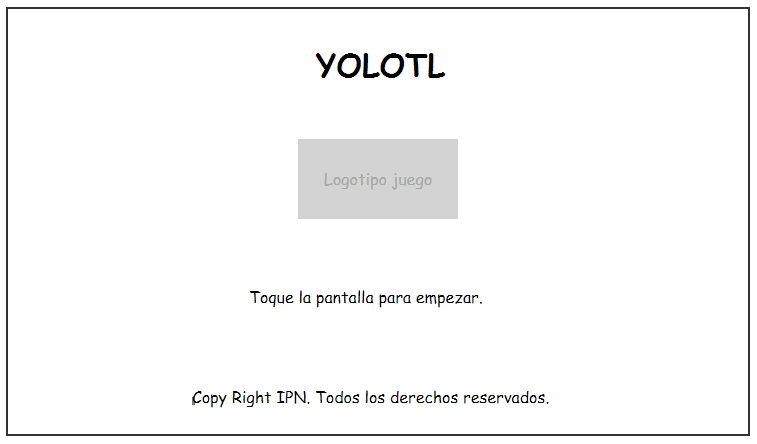
\includegraphics[width=0.6 \textwidth]{05TrabajoRealizado/01DocDiseno/Interfaz/imagenes/interfaz00}
  \caption{Interfaz 1.0 Pantalla de inicio.}
  \label{fig:PInicio}
\end{figure} 

Ver figura \ref{fig:PInicio}

\subsubsection{Interfaz 2.00 Menú principal.} \label{inter:interfaz02}
	\subsubsection{Descripción de la pantalla}
El logotipo del juego se muestra en la parte superior derecha de la pantalla. En la parte inferior izquierda se muestran las dos opciones: Nueva partida, Cargar partida. De fondo se muestra la misma Imagen que en la interfaz 01.00. 
Cada opción desencadena un cuadro de dialogo en donde el usuario debe de confirmar la acción que va desea ejecutar o en donde se le informa que la acción seleccionada no es posible de ejecutar.
	\subsubsection{Estados del juego}
La interfaz 2.00 contiene los siguientes botones:
\begin{itemize}
	\item \textbf{Nueva partida}:  Dirige a la presentación de la cinemática 1 (ver apartado \ref{Cin:Cinematica01}).
	\item \textbf{Cargar partida}: Dirige a la interfaz 3.00 (ver apartado \ref{inter:interfaz03}) en caso de que exista una partida previamente guardada, en caso contrario abre un cuadro de dialogo en donde se le dice al Jugador que no existe partidas que cargar.
\end{itemize}
Se puede llegar a esta Interfaz a partir de la Interfaz 01.00 (ver apartado \ref{inter:interfaz01})
	\subsubsection{Imagen}
Ver figura \ref{fig:PMenuP}
\begin{figure}
  \centering
   \subfigure[Menú principal] {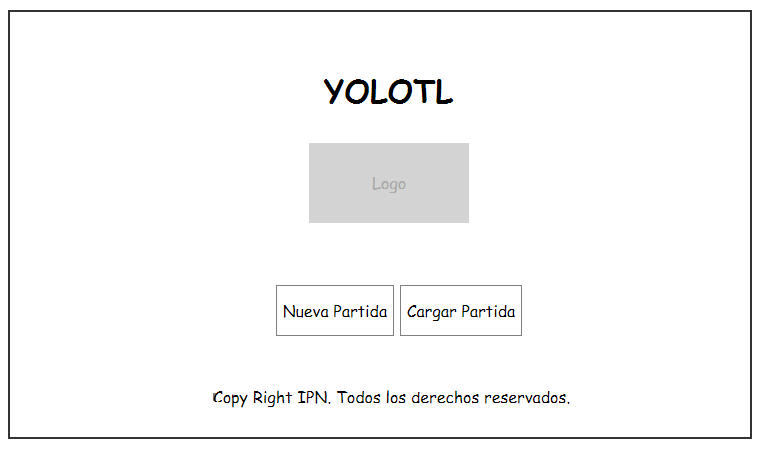
\includegraphics[width=0.6 \textwidth]{05TrabajoRealizado/01DocDiseno/Interfaz/imagenes/interfaz01}}
   
 	\subfigure[Cuadro de dialogo para confirmar iniciar nueva partida.] {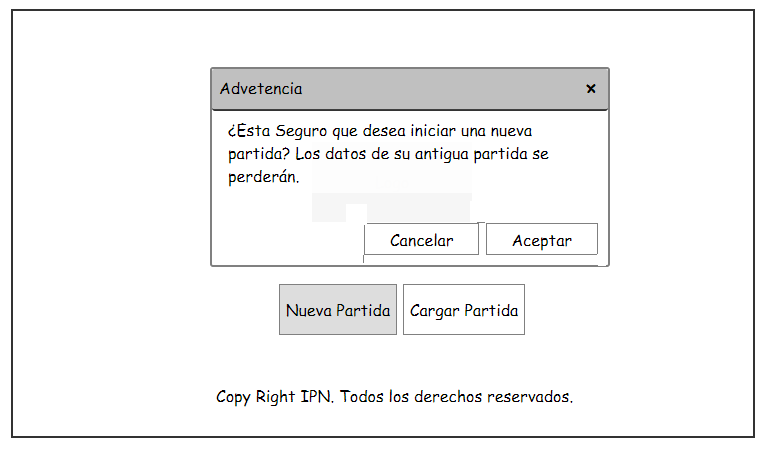
\includegraphics[width=0.6 \textwidth]{05TrabajoRealizado/01DocDiseno/Interfaz/imagenes/interfaz01_02}}
 	
\subfigure[Cuadro de dialogo cuando no existen partidas que cargar.] {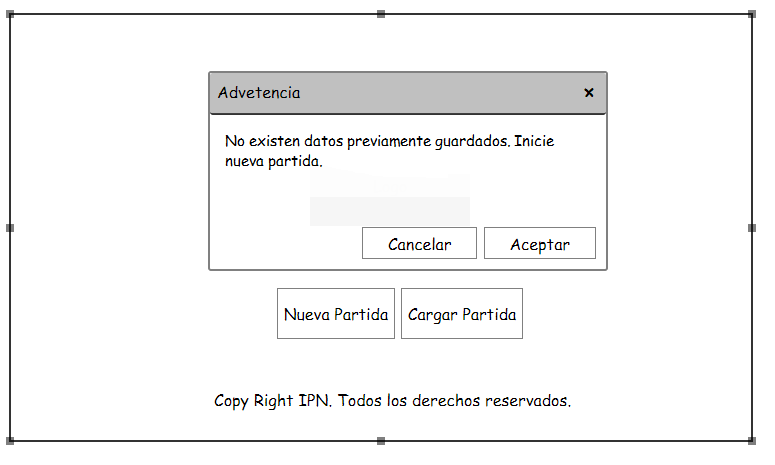
\includegraphics[width=0.6 \textwidth]{05TrabajoRealizado/01DocDiseno/Interfaz/imagenes/interfaz01_03}}
  \caption{Interfaz 2.00 Menú principal.}
  \label{fig:PMenuP}
\end{figure} 
\section{Interfaz 3.00 Selección de nivel}\label{inter:interfaz03}
	\subsection{Descripción de la pantalla}
Muestra el nombre de la pantalla en la esquina superior izquierda.
Los iconos de nivel y de las cinemáticas estarán organizados en un carrusel que permitirá su selección. Los niveles y cinemáticas disponibles a elegir en el carrusel dependerán de la carga automática. Los niveles disponibles disponibles para jugar mostrarán una imagen descriptiva en el carrusel mientras que los niveles no disponibles mostraran un imagen de un cuadro negro.   
Bajo el carrusel se encontrara un apartado donde se podrá visualizar información del nivel seleccionado en el carrusel, tal como el nombre y una breve descripción.
El botón que permite iniciar una partida en el nivel seleccionado se encontrará ubicado al lado derecho de la sección donde se muestra la información del nivel. 
	\subsection{Estados del juego}
Se llega a esta interfaz a través de la interfaz 2.00 (ver apartado\ref{inter:interfaz02}), siempre que el Jugador oprima el botón de cargar partida.
La interfaz 3.0 cuenta con los siguientes botones:
\begin{itemize}
	\item \textbf{Iniciar Nivel}: Envía al inicio del nivel seleccionado.
	\item \textbf{Control de carrusel}: estos botones permite controlas los elementos que se almacenan en el carrusel.
\end{itemize} 
	\subsection{Imagen}
	Ver figura \ref{fig:SelNivel}
\begin{figure}
  \centering
   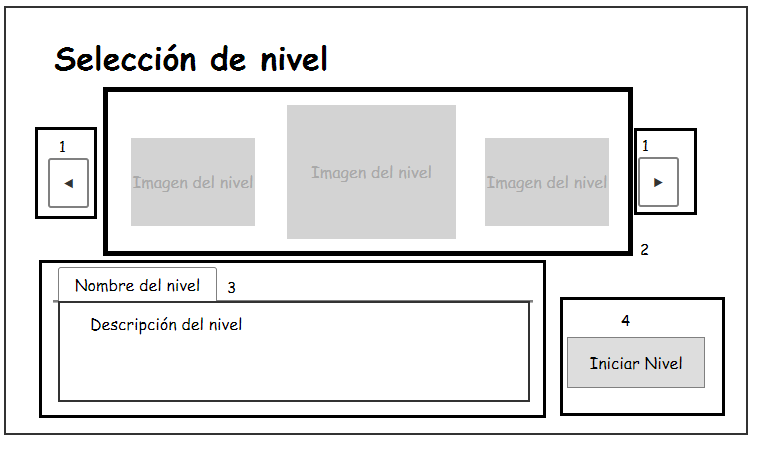
\includegraphics[width=0.6 \textwidth]{Imagenes/interfaz02_01}
  \caption{Interfaz 2.00 Selección de nivel.1 botones que controlan el carrusel. 2 Carrusel. 3 Información del nivel seleccionado. 4 Botón Iniciar nivel.}
  \label{fig:SelNivel}
\end{figure} 